% lecture15.tex — Oriented Intersection Number

\section{Oriented Intersection Number}

Consider oriented manifolds $M, N, P$, with $M$ compact, $P \subset N$ closed, and
\[
    \dim M + \dim P = \dim N.
\]

If $f \colon M \to N$ is transversal to $P$, then $f^{-1}(P)$ is a finite number of points, each with an orientation number $\in \{\pm 1\}$.

\begin{definition}{Intersection Number}{intersection-number}
    The \emph{intersection number} $I(f, P) \in \Z$ is defined to be the sum of these orientation numbers.
\end{definition}

The orientation number at $x \in f^{-1}(P)$ is $+1$ (resp.\ $-1$) if the isomorphism
\[
    df_x(T_x M) \oplus T_{f(x)} P = T_{f(x)} N
\]
is orientation preserving (resp.\ reversing). Note, the ordering is important!

\begin{example}{Circles on a Torus}{torus-circles}
    For the two standard circles $C_1, C_2$ on a torus, $I(C_1, C_2) = 1$ and $I(C_2, C_1) = -1$.
\end{example}

\begin{center}
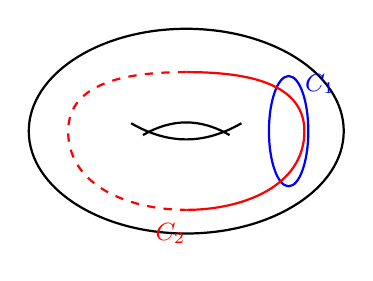
\begin{tikzpicture}[scale=1]
    % Torus outline
    \draw[thick] (0,0) ellipse (2 and 1.3);
    % Inner hole
    \draw[thick] (-0.7,0.1) to[out=-30,in=210] (0.7,0.1);
    \draw[thick] (-0.55,-0.05) to[out=30,in=150] (0.55,-0.05);
    % Meridian C_1 (goes around the tube)
    \draw[thick,blue] (1.3,0) ellipse (0.25 and 0.7);
    \node[blue] at (1.7,0.6) {\small $C_1$};
    % Longitude C_2 (goes around the hole)
    \draw[thick,red] (0,-1.0) to[out=0,in=-90] (1.5,0) to[out=90,in=0] (0,0.75);
    \draw[thick,red,dashed] (0,0.75) to[out=180,in=90] (-1.5,0) to[out=-90,in=180] (0,-1.0);
    \node[red] at (-0.2,-1.3) {\small $C_2$};
\end{tikzpicture}
\end{center}

\begin{proposition}{Vanishing on Boundaries}{intersection-boundary-zero}
    If $M = \partial W$ for some compact, oriented $W$ and $f \colon M \to N$ extends to $W$, then $I(f, P) = 0$ for any closed $P \subset N$ of complementary dimension.
\end{proposition}

\begin{proof}
    The proof is the same as the analogous theorem in mod 2 intersection theory. Here, $F^{-1}(P)$ is a compact oriented 1-manifold, so the signed count of $\partial F^{-1}(P)$ is $0$.
\end{proof}

\begin{center}
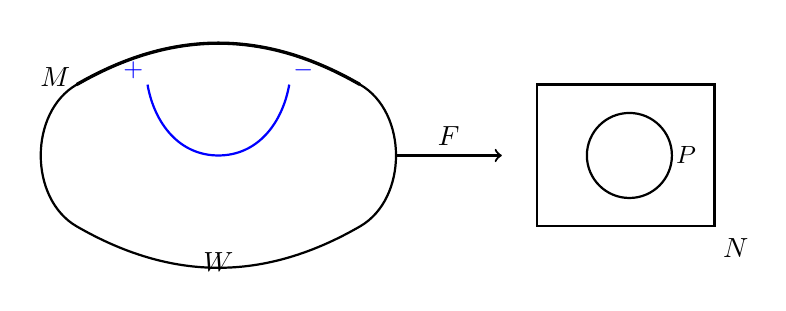
\begin{tikzpicture}[scale=0.9]
    % W (blob) with M = boundary
    \draw[thick] (0,0) to[out=30,in=150] (4,0) to[out=-30,in=30] (4,-2) to[out=210,in=330] (0,-2) to[out=150,in=210] cycle;
    \node at (2,-2.5) {$W$};
    \draw[very thick] (0,0) to[out=30,in=150] (4,0);
    \node at (-0.3,0.1) {$M$};
    % F^{-1}(P) arc with signed endpoints
    \draw[thick,blue] (1,0) to[out=-80,in=180] (2,-1) to[out=0,in=260] (3,0);
    \node[blue] at (0.8,0.2) {\small $+$};
    \node[blue] at (3.2,0.2) {\small $-$};
    % Arrow + F label to right
    \draw[->,thick] (4.5,-1) -- (6,-1) node[midway,above] {$F$};
    % N with P inside
    \draw[thick] (6.5,-2) rectangle (9,0);
    \node at (9.3,-2.3) {$N$};
    \draw[thick] (7.8,-1) circle (0.6);
    \node at (8.6,-1) {\small $P$};
\end{tikzpicture}
\end{center}

\begin{proposition}{Homotopy Invariance}{intersection-homotopy}
    Homotopic maps have the same intersection numbers.
\end{proposition}

\begin{proof}
    The proof is analogous to the mod 2 case. If $F \colon I \times M \to N$ is a homotopy between $f_0, f_1 \colon M \to N$, then
    \[
        0 = I(\partial F, P) = I(f_1, P) - I(f_0, P),
    \]
    since $\partial(I \times M) = M_1 - M_0$, so $\partial F^{-1}(P) = f_1^{-1}(P) - f_0^{-1}(P)$.
\end{proof}

\subsection{Degree}

In the same manner, when $N$ is connected and $\dim N = \dim M$, we define the \emph{degree} of $f \colon M \to N$ to be
\[
    \deg(f) = I(f, \{y\}),
\]
for any (positively oriented) point $y \in N$.

\begin{example}{Winding Number}{winding-number}
    The winding number of a closed curve in the plane around a point is a degree.
\end{example}

\begin{center}
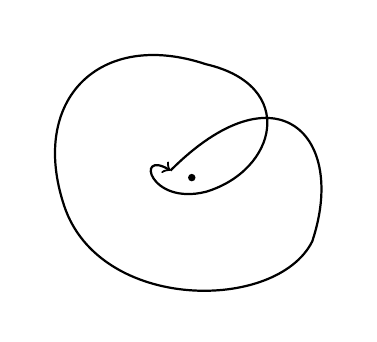
\begin{tikzpicture}[scale=0.9]
    % A closed curve winding around a point
    \draw[thick,->] (0,0) .. controls (1.5,1.5) and (2.5,0.5) .. (2,-1)
        .. controls (1.5,-2) and (-1,-2) .. (-1.5,-0.5)
        .. controls (-2,1) and (-1,2) .. (0.5,1.5)
        .. controls (1.8,1.2) and (1.5,0) .. (0.5,-0.3)
        .. controls (-0.3,-0.5) and (-0.5,0.3) .. (0,0);
    \fill (0.3,-0.1) circle (1.5pt);
\end{tikzpicture}
\end{center}

\begin{example}{Degree of $z \mapsto z^m$}{degree-power}
    The map $S^1 \to S^1$, $z \mapsto z^m$, has degree $m \in \Z$. In particular, $z^m$ and $z^{m'}$ (as maps $S^1 \to S^1$) are not homotopic whenever $m \neq m'$.
\end{example}

\subsection{Reformulation via the Diagonal}

The following reformulation is useful.

Let $M_1, M_2$ be compact with $\dim M_1 + \dim M_2 = \dim N$. For any $f_1 \colon M_1 \to N$ and $f_2 \colon M_2 \to N$, we say they are \emph{transversal}, $f_1 \pitchfork f_2$, if
\begin{equation}
    (df_1)_{x_1}(T_{x_1} M_1) \oplus (df_2)_{x_2}(T_{x_2} M_2) = T_y N \tag{$*$}
\end{equation}
whenever $f_1(x_1) = y = f_2(x_2)$.

Basic linear algebra shows $f_1 \pitchfork f_2 \iff f_1 \times f_2 \pitchfork \Delta$, where $f_1 \times f_2 \colon M_1 \times M_2 \to N \times N$ and $\Delta \subset N \times N$ is the \emph{diagonal}.

Define $I(f_1, f_2)$ to be the sum of local intersection numbers, each of which is given by $+1$ (resp.\ $-1$) if the isomorphism ($*$) is orientation preserving (resp.\ reversing).

\begin{proposition}{Intersection via Diagonal}{intersection-diagonal}
    \[
        I(f_1, f_2) = (-1)^{\dim(M_2)} \, I(f_1 \times f_2, \Delta).
    \]
\end{proposition}

\begin{proof}
    This is linear algebra again. Let $U = (df_1)_{x_1}(T_{x_1} M_1)$ and $V = (df_2)_{x_2}(T_{x_2} M_2)$, and let $\{u_1, \ldots, u_k\}$ and $\{v_1, \ldots, v_\ell\}$ be their positively oriented ordered bases. We may assume $\{u_1, \ldots, u_k, v_1, \ldots, v_\ell\}$ is positively oriented for $T_y N$. Then, for $U \times V$,
    \begin{align*}
        &\sign\{(u_1, 0), \ldots, (u_k, 0), (0, v_1), \ldots, (0, v_\ell), (u_1, u_1), \ldots, (u_k, u_k), (v_1, v_1), \ldots, (v_\ell, v_\ell)\} \\
        &\qquad = \sign\{(u_1, 0), \ldots, (u_k, 0), (0, v_1), \ldots, (0, v_\ell), (0, u_1), \ldots, (0, u_k), (v_1, 0), \ldots, (v_\ell, 0)\} \\
        &\qquad = (-1)^{\ell(\ell + k) + \ell k} \sign\{(u_1, 0), \ldots, (v_\ell, 0), (0, u_1), \ldots, (0, v_\ell)\} \\
        &\qquad = (-1)^\ell.
    \end{align*}
\end{proof}

\begin{proposition}{Homotopy Invariance of Pairs}{intersection-pairs-homotopy}
    If $f_0$ and $g_0$ are homotopic to $f_1$ and $g_1$, respectively, then $I(f_0, g_0) = I(f_1, g_1)$.
\end{proposition}

\begin{proof}
    $f_t \times g_t$ is a homotopy between $f_0 \times g_0$ and $f_1 \times g_1$.
\end{proof}

In particular, if $M_1, M_2 \subset N$ are compact submanifolds of complementary dimension, then $I(M_1, M_2)$ is invariant under homotopy of either $M_1$ or $M_2$.

Note, from the definition,
\[
    I(M_1, M_2) = (-1)^{(\dim M_1)(\dim M_2)} I(M_2, M_1).
\]

\subsection{Euler Characteristic}

\begin{definition}{Euler Characteristic}{euler-characteristic}
    If $M$ is a compact, orientable manifold, its \emph{Euler characteristic} $\chi(M)$ is defined to be $I(\Delta, \Delta)$, where $\Delta \subset M \times M$ is the diagonal.
\end{definition}

We immediately have:

\begin{proposition}{Odd-Dimensional Euler Characteristic}{odd-dim-euler}
    The self-intersection number of any odd-dimensional compact oriented manifold is $0$. In particular, $\chi(M) = 0$ for any odd-dimensional compact oriented manifold.
\end{proposition}

Recall that $I_{\Z/2}(C, C) = 1$ for the central circle $C$ in the M\"obius strip. This shows that the M\"obius strip is \emph{not orientable} (for if it were, then $I_{\Z/2}(C, C) = I(C, C) \mod 2 = 0$).
